\section{Results}\label{sec:results}
\subsection{Run selection}
On the common selection set (\RCmpN{} images), run 2 reached macro-F1 \RCmpRunTwoMacroFOne\% against
\RCmpRunOneMacroFOne\% for run 1, accuracy \RCmpRunTwoAcc\% against \RCmpRunOneAcc\%, and macro ROC-AUC
\RCmpRunTwoMacroAUC{} against \RCmpRunOneMacroAUC. Run 1 was right and run 2 wrong on \RCmpMcNemarB{}
images, the reverse on \RCmpMcNemarC{} (exact McNemar $p{=}\RCmpMcNemarP$, descriptive only). On the
\RCmpRunOneSharedN{} common images from the four sources both runs trained on, accuracy is almost equal
(\RCmpRunOneSharedAcc\% against \RCmpRunTwoSharedAcc\%) and the macro-F1 gap is smaller
(\RCmpRunOneSharedMacroFOne\% against \RCmpRunTwoSharedMacroFOne\%). Much of run 2's advantage therefore lies on
TBX11K and COVID-19 Radiography images, which are in-distribution for run 2 only.

\subsection{Internal test}
On the test split of \RNTest{} images the selected model reaches \RTestAcc\% accuracy (bootstrap interval
\RTestAccLo--\RTestAccHi\%), macro-F1 \RTestMacroFOne\%, macro ROC-AUC \RTestMacroAUC{} and ECE \RTestECE;
validation accuracy was \RValAcc\%. The earlier leaky V5 model reported \RVFiveAcc\% on a different test
set (N=\RVFiveN); the numbers are not comparable. Table~\ref{tab:perclass} gives per-class results and
Fig.~\ref{fig:cm} the confusion matrix. COVID-19 (F1 \RFOneCovid\%), Tuberculosis (\RFOneTB\%) and
Pneumonia (\RFOnePneumonia\%) are the strongest classes. Pulmonary Nodule/Mass is the weakest (\RFOneNodule\%),
followed by Normal (\RFOneNormal\%). Nodule/Mass and Pleural Effusion are NIH-only classes with
language-mined labels.

\begin{table}[t]
\caption{Per-class test results (single run, seed \RSeed): support (N), precision (P), recall (R) and F1 in \%;
one-vs-rest ROC-AUC.}
\label{tab:perclass}
\centering
\small
\begin{tabular}{lrrrrr}
\toprule
Class & N & P & R & F1 & AUC\\
\midrule
COVID-19 & \RSupportCovid & \RPrecisionCovid & \RRecallCovid & \RFOneCovid & \RAUCCovid\\
Normal & \RSupportNormal & \RPrecisionNormal & \RRecallNormal & \RFOneNormal & \RAUCNormal\\
Pleural Effusion & \RSupportEffusion & \RPrecisionEffusion & \RRecallEffusion & \RFOneEffusion & \RAUCEffusion\\
Pneumonia & \RSupportPneumonia & \RPrecisionPneumonia & \RRecallPneumonia & \RFOnePneumonia & \RAUCPneumonia\\
Nodule / Mass & \RSupportNodule & \RPrecisionNodule & \RRecallNodule & \RFOneNodule & \RAUCNodule\\
Tuberculosis & \RSupportTB & \RPrecisionTB & \RRecallTB & \RFOneTB & \RAUCTB\\
\bottomrule
\end{tabular}
\end{table}

\begin{figure}[t]
\centering
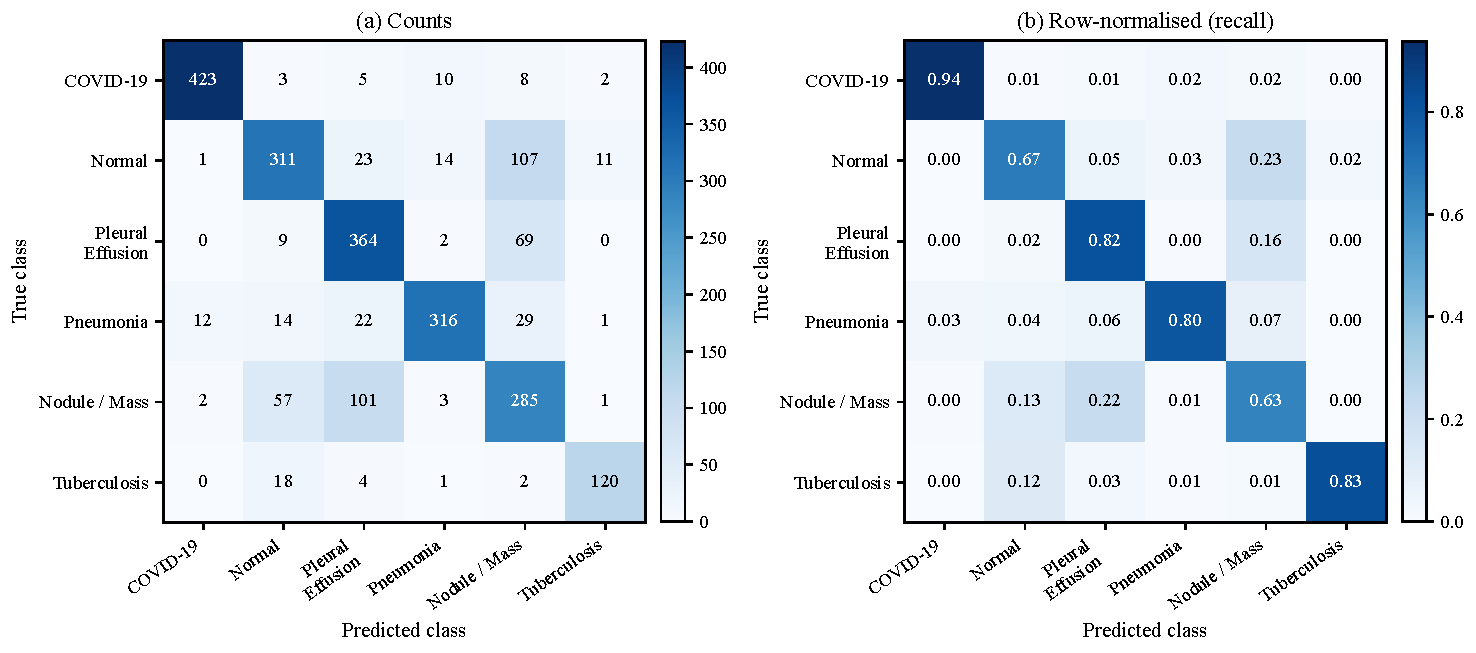
\includegraphics[width=\columnwidth]{../../figures/fig_confusion_matrix.pdf}
\caption{Test confusion matrix (counts and row-normalised).}
\label{fig:cm}
\end{figure}

\subsection{External validation (Montgomery County)}
On the \RNExternal{} external scans the model flags \RExtSensK/\RExtSensN{} TB scans as abnormal
(\RExtSens\%, Wilson interval \RExtSensLo--\RExtSensHi\%), calls \RExtSpecK/\RExtSpecN{} normal scans Normal
(\RExtSpec\%, interval \RExtSpecLo--\RExtSpecHi\%), and names \RExtTBK/\RExtTBN{} TB scans Tuberculosis
(\RExtTB\%). The ROC-AUC of the abnormality score is \RExtAUC. Most scans are assigned to Pneumonia and
Pulmonary Nodule/Mass (Fig.~\ref{fig:ext}); only \RExtCovidCalls{} are called COVID-19. The low specificity
means the model would flag most healthy patients from this hospital as abnormal.

The first run behaved differently. Run 1 called \RRunOneExtCovidCalls{} of \RNExternal{} Montgomery scans COVID-19 and \RRunOneExtSpecK{} of \RExtSpecN{} normal scans
Normal (each run evaluated once).
Run 2 calls \RExtCovidCalls{} scans COVID-19 and \RExtSpecK{} of \RExtSpecN{} normals Normal. Adding a large
second COVID-19 source thus removed the run-1 COVID-19 pattern, but the errors moved to other abnormal
classes: internal gains did not translate into better external specificity or any TB recognition.

\begin{figure}[t]
\centering
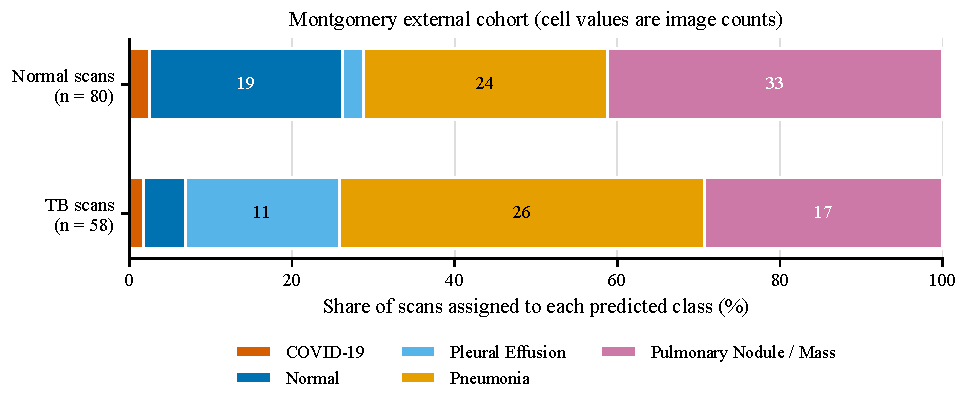
\includegraphics[width=\columnwidth]{../../figures/fig_external_breakdown.pdf}
\caption{Montgomery County: predicted class for normal and TB scans (selected model).}
\label{fig:ext}
\end{figure}

\subsection{Source effects}
Test accuracy differs by source (Table~\ref{tab:source}): it is lowest for Cohen and NIH images and highest for
the COVID-19 Radiography images. We do not read this as a ranking of data quality. Sources differ in
which classes they contain, so source and class are confounded.

\begin{table}[t]
\caption{Test accuracy by source (N images, accuracy in \%).}
\label{tab:source}
\centering
\small
\begin{tabular}{lrr}
\toprule
Source & N & Accuracy\\
\midrule
NIH ChestX-ray14 & \RSrcNNIH & \RSrcAccNIH\\
Kermany & \RSrcNKermany & \RSrcAccKermany\\
COVID-19 Radiography & \RSrcNCovidRad & \RSrcAccCovidRad\\
TBX11K & \RSrcNTBXk & \RSrcAccTBXk\\
Cohen & \RSrcNCohen & \RSrcAccCohen\\
Shenzhen & \RSrcNShenzhen & \RSrcAccShenzhen\\
\bottomrule
\end{tabular}
\end{table}
